\subsection{Synthesizing Path-compliant  Inter-domain Configurations}
\label{sec:inter-synthesis}

Next, we extend our algorithm to
solve the path-compliance problem in the presence
of multiple domains---i.e., $|\{\Theta(r) \mid r\in V\}|>1$.
First, our algorithm determines the 
BGP configuration and static routes to ensure that the 
paths will traverse the correct domains.
Second, we show how to modify the 
techniques given in Section~\ref{sec:intra-synthesis}
to determine the edge weights and static routes
 in each domain to guarantee that paths traverse
the correct gateway routers.


\subsubsection{Configuring BGP and Static Routes}
BGP is a path-vector protocol where each BGP router,
for each destination $\lambda$,
advertises to its peers
what sequence of domains one should follow to get to  $\lambda$.  
In this section, we describe how to configure
BGP routers so that the routes chosen by BGP 
(and redistributed into OSPF) 
can yield the policy-compliant
paths $\Pi$ given as input. 
We need to take into account three different
cases, which are illustrated in \Cref{fig:bgpexample}.  
For sake of simplicity, we omit certain small details 
from the following discussion.

In the first case, a path is preferred because it traverses fewer domains.
For example, in \Cref{fig:bgpexample}(a), we want
path (1)---i.e., the red one---to be the chosen path from source $s$ 
to destination $\lambda$.
Here, BGP router $g_3$ receives from $g_6$ an advertisement for a route to destination $\lambda$
traversing only the domain $1$; this route has domain path length 1 as it only traverses 1 domain. 
Instead, $g_1$ and $g_2$ receive advertisements for a route 
(D2, D1)
to destination $\lambda$  with 
domain path length 2. Since our objective is to send traffic along
$g_3$, for path (1) we do not need to add any further BGP configurations,
and the route via $g_3$ is automatically redistributed into domain D0;
for destination $\lambda$, the gateway at domain D0 is $g_3$, i.e.,
$G(0, \lambda) = g_3$.

In the second case, the requested path does not have shortest domain path length
and we therefore need to set local preferences.
For example, let's say that in \Cref{fig:bgpexample}(a) we now want
path (2)---i.e., the purple one---to be the chosen path from source $s$
to destination $\lambda$. 
Since $g_1$'s route traverses more domains than
 $g_3$'s route,
we need to set the local preference of route received by $g_1$ 
(from $g_4$) to a value greater than the preference for the route received by $g_3$. 
In the example, we set the preference at node $g_1$: 
$LP(g_1, g_4, \lambda) = 100$
which causes $g_1$ to become gateway at domain D0 for destination $\lambda$, i.e., 
$G(0, \lambda) = g_1$.

In the third case, two paths from different sources 
destination $\lambda$ exit
the domain through two different
gateways.
For example, in \Cref{fig:bgpexample}(b),
the path from $r_1$ to $\lambda$ exits domain D0 through 
gateway router $g_1$, while the path from $r_2$  to $\lambda$ exits 
through $g_2$. 
Moreover,  we assume that $g_1$ is the closest gateway to $r_1$ and 
$g_2$ is the closest gateway to $r_2$ w.r.t. OSPF paths in the domain.
In this case, both these routes need to be  
redistributed to the OSPF domain. 
By assigning local preferences such that
$LP(g_1,g_3,\lambda)<LP(g_2,g_4,\lambda)$,
 $g_2$ will redistribute a route for $\lambda$ 
 to the OSPF domain and
the traffic from $r_2$ will correctly exit through $g_2$. 
To prevent the traffic from $r_1$ to exit through $g_2$,
we add an iBGP filter
\footnote{Gateways $g_1$ and $g_2$ need not be connected by a physical 
	link directly; iBGP establishes a connection among the 
	BGP routers in a domain.}
 for the connection $g_2 \rightarrow g_1$ for
destination IP $\lambda$. 
Thus, $g_1$ will not receive the
a route for $\lambda$ from $g_2$, and therefore,
redistribute the route it received from $g_3$. For 
this example, $G(0, \lambda) = \{g_1, g_2\}$.
$\lambda$ traffic from $r_1$ will exit through $g_1$ 
as it is the closest gateway. 

\begin{figure*}
	\centering
	\subfloat[Single
	BGP Gateway]{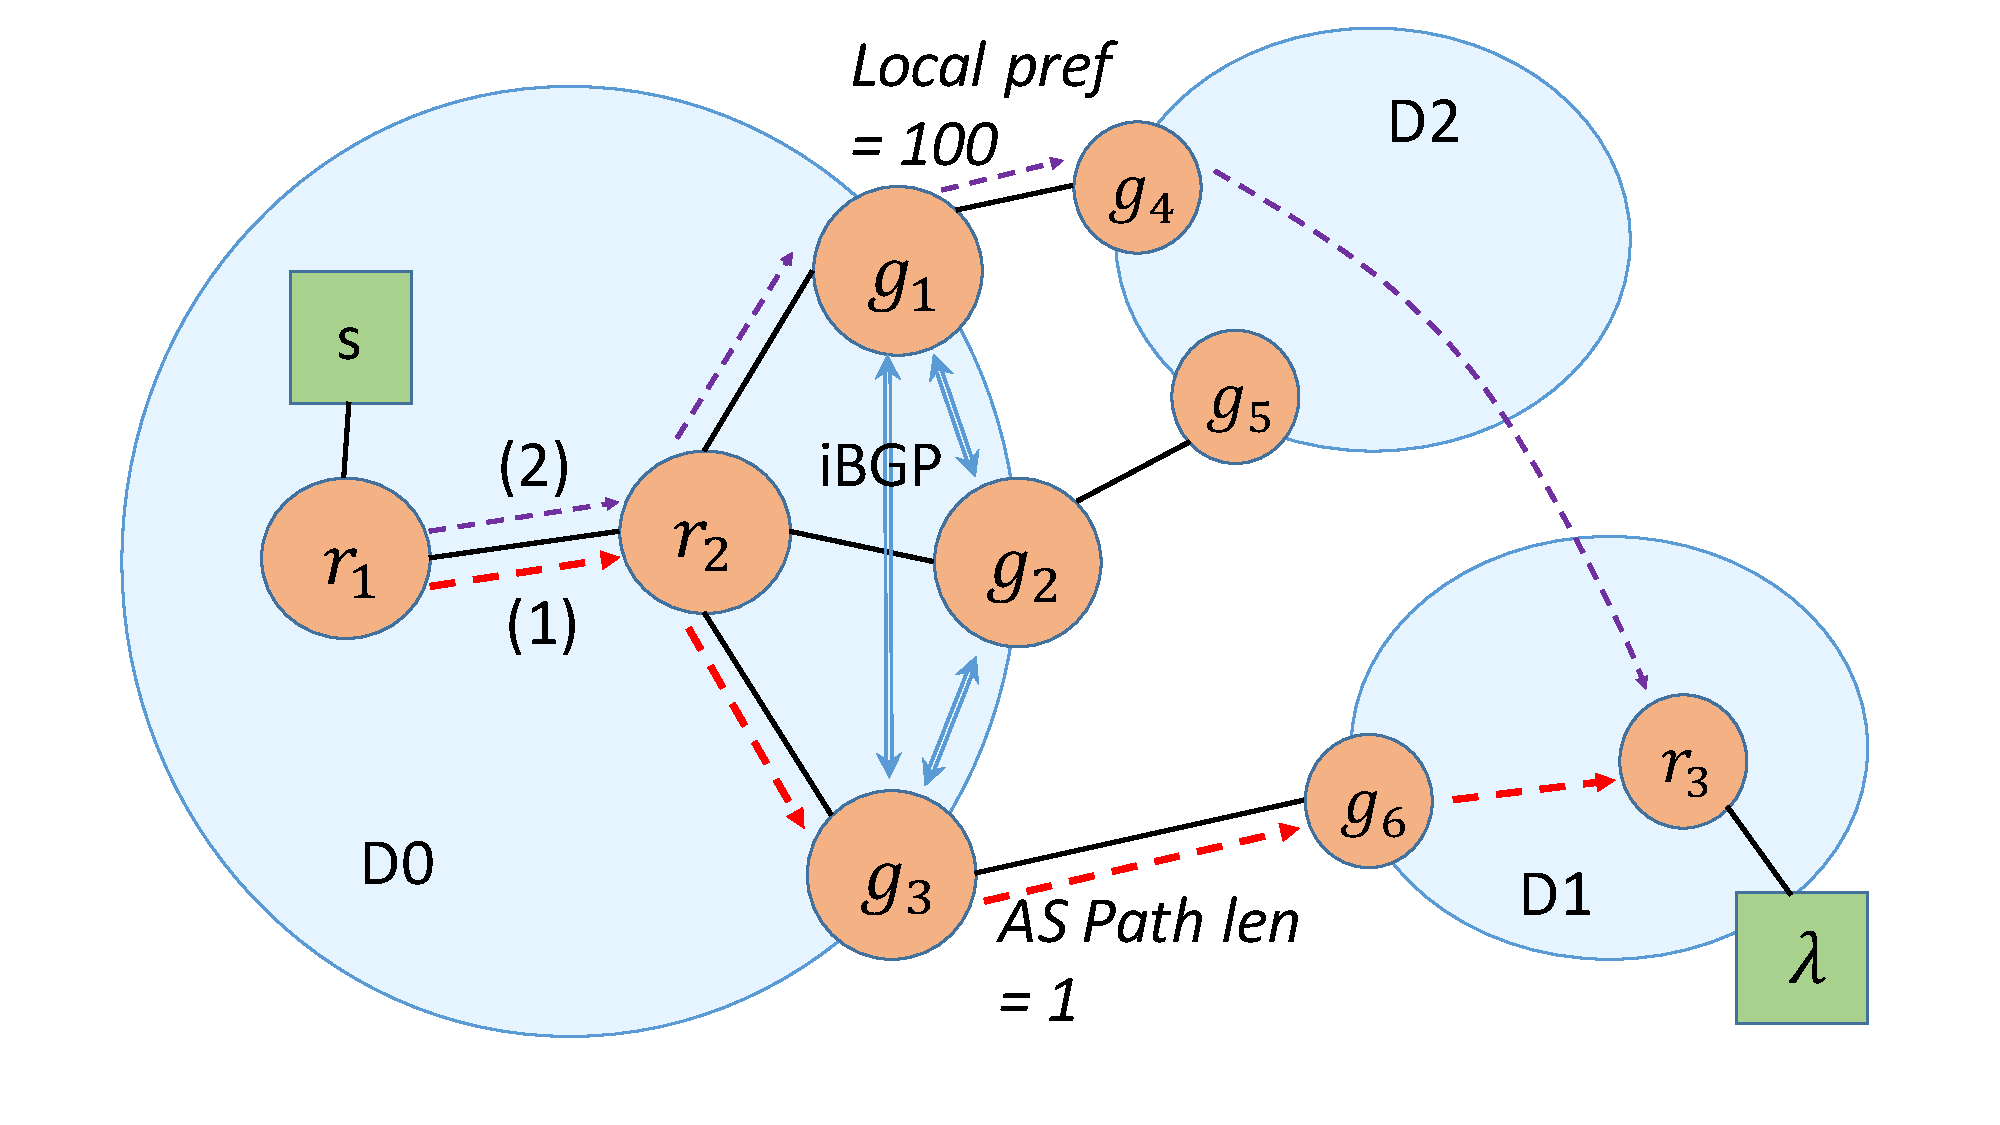
\includegraphics[width=0.305\columnwidth]{figures/bgp-example.pdf}}
	\hfill
	\subfloat[Multiple BGP Gateways]{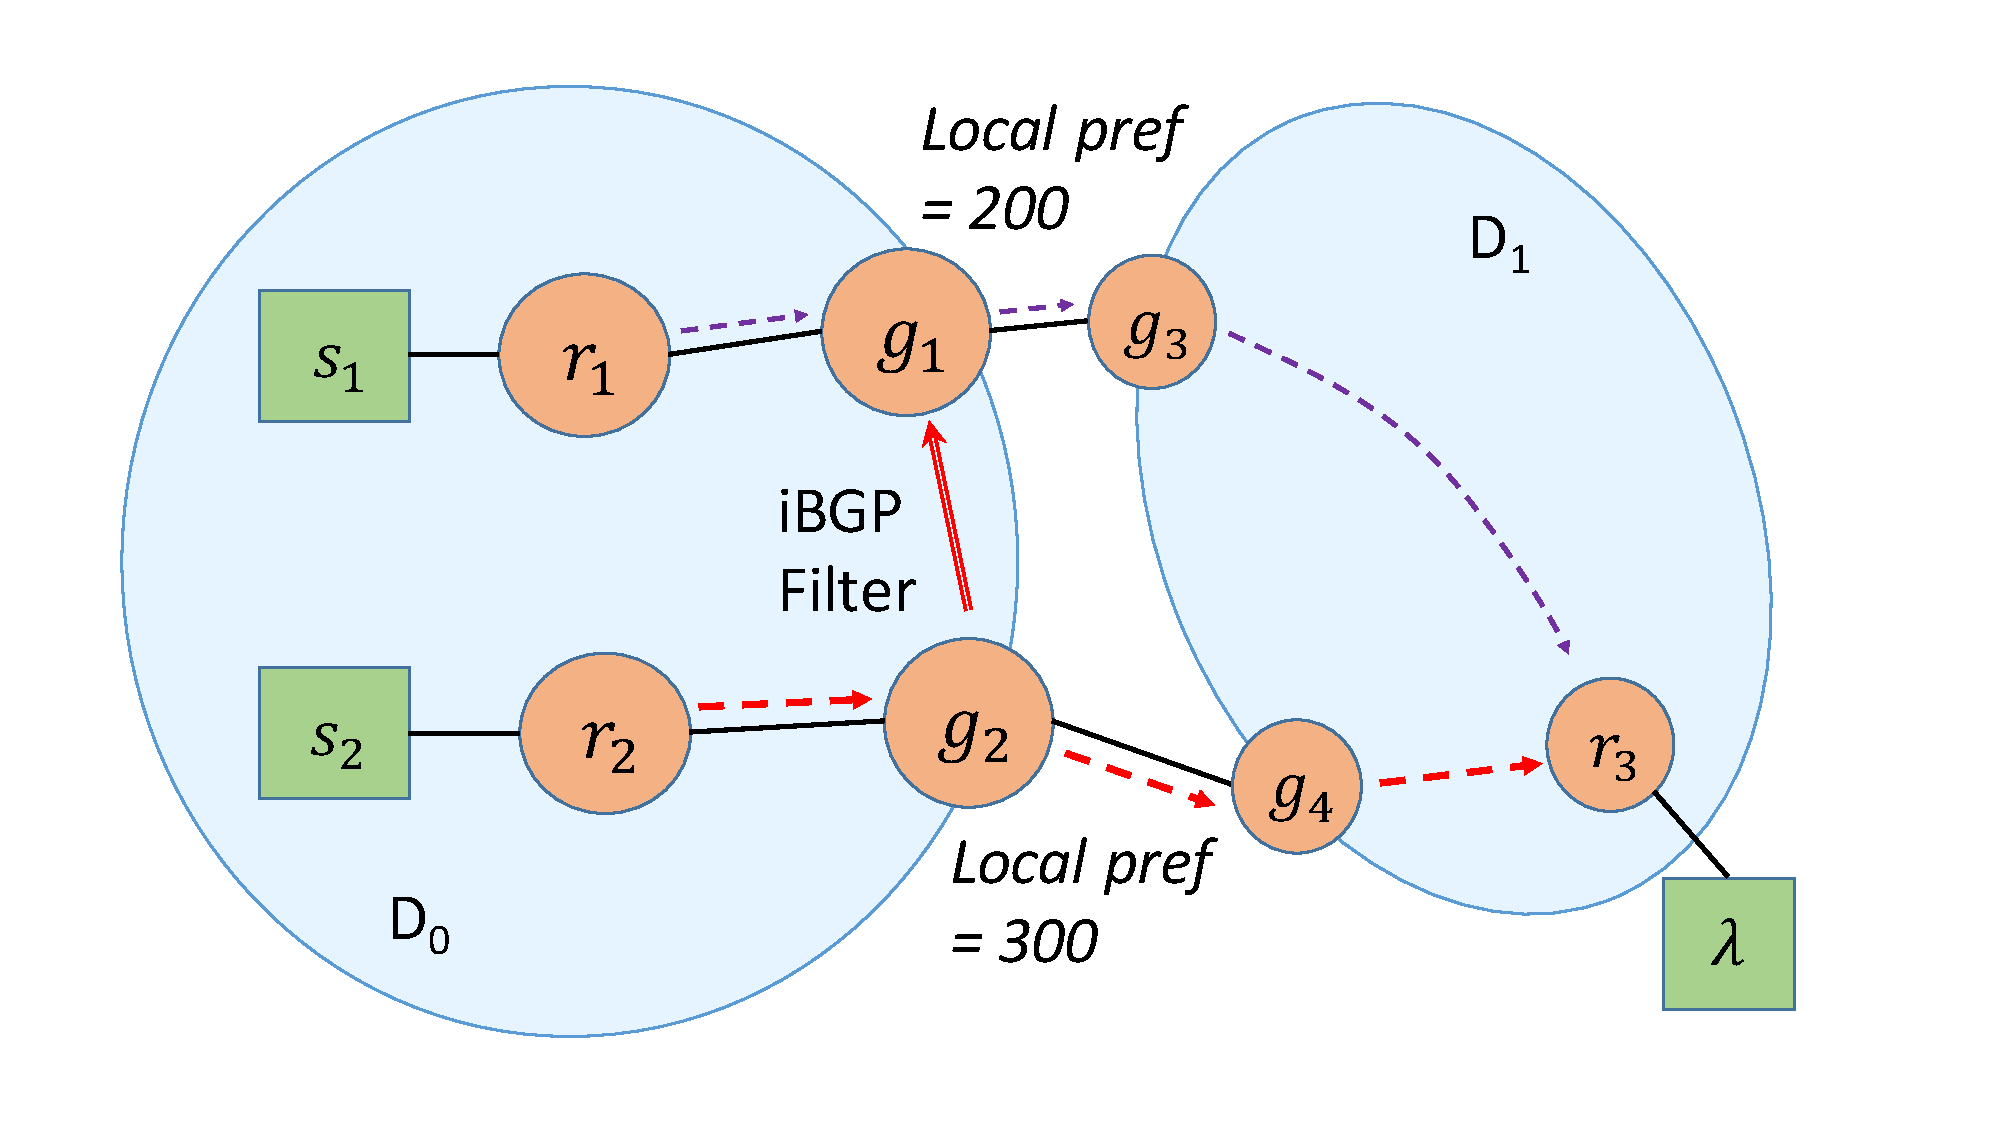
\includegraphics[width=0.33\columnwidth]{figures/bgp-example2.pdf}}
	\hfill
	\subfloat[Static Routes]{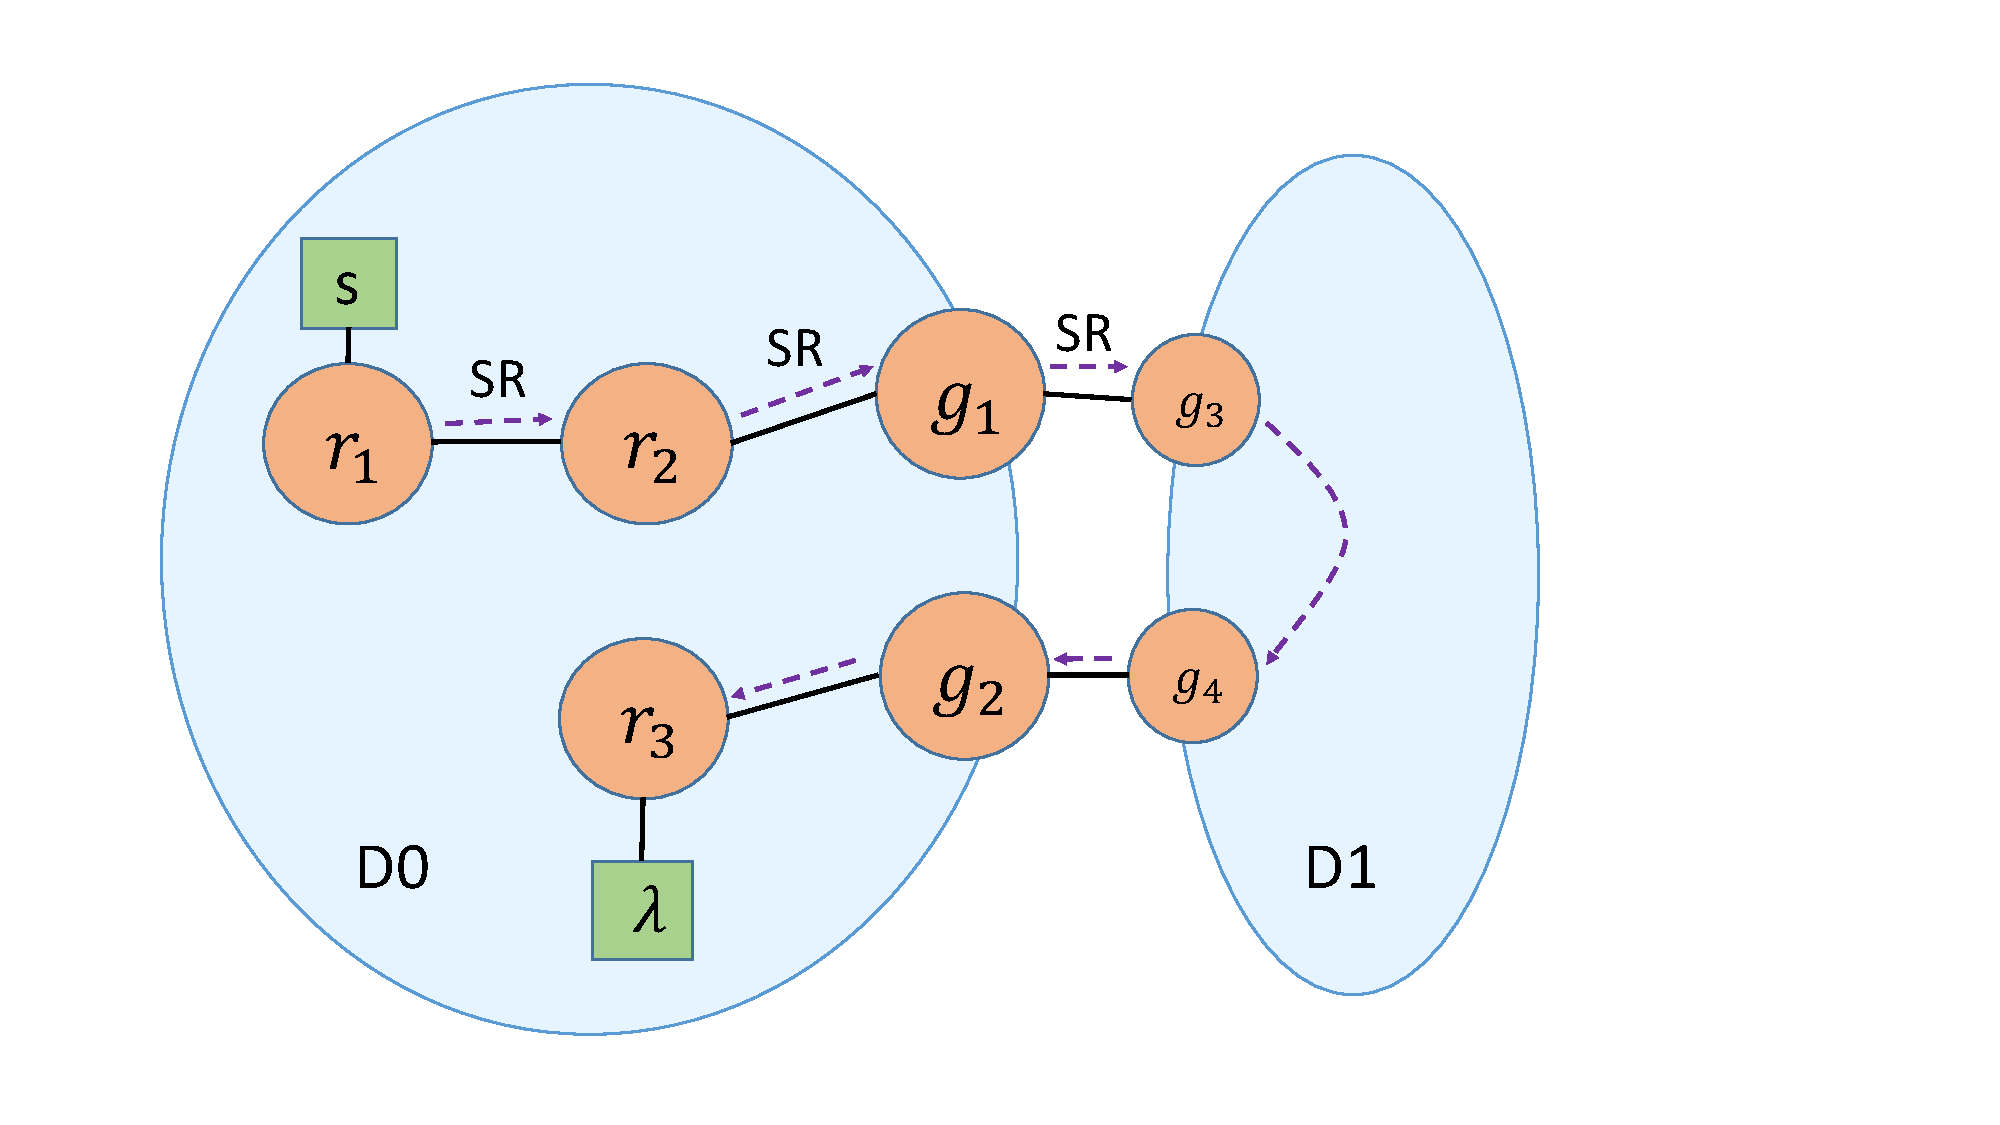
\includegraphics[width=0.265\columnwidth]{figures/static-route.pdf}}
	\compactcaption{\label{fig:bgpexample}
		Examples of BGP and static route configurations for 
		inter-domain routing given domain assignment $\Theta$.}
\end{figure*}

%\minisection{Static Routes} \label{sec:static}
Finally, we describe a case in which standard BGP cannot enforce
the desired path, therefore requiring the use of static routes.
Consider the path for destination $\lambda$ 
shown in \Cref{fig:bgpexample}(c). BGP Gateway $g_1$, which is in
domain D0, 
will receive an advertisement for $\lambda$ that goes through domain
1 and then domain D0.
This advertisement will be rejected because it creates a loop---i.e., the domain D0
appears twice in the path. 
To enforce domain paths with loops, we use static routes. In this example
the static routes
$SR(r_1,\lambda) = \{r_2\}$, $SR(r_2,\lambda) = \{g_1\}$, and $SR(g_1,\lambda) = \{g_2\}$ 
guarantee that routes from $r_1$, $r_2$, and $g_2$ to $\lambda$ traverse the desired links.

\minisection{Algorithm}
We are now ready to describe the algorithm that,
given a set of paths $\Pi$, determines
BGP local preferences, iBGP filters, and static routes for enforcing such paths.
For a path $\pi = l_1 l_2 \ldots l_m \in \Pi$, we
can divide the path into intra-domain paths and inter-domain
links. We express $\pi$ as 
$\pi_1 idl_1^2 \pi_2 \ldots idl_{n-1}^n \pi_n$ where
each subpath $\pi_i$ is completely in a
domain, i.e., for each 
link $(r_1,r_2) \in \pi_i \implies \Theta(r_1) = \Theta(r_2)$;
and links $idl_1^2, idl_2^3 \ldots idl_{n-1}^n$ 
represent the inter-domain links, i.e., 
if $idl_i^{i+1}=(r,r')$ then $\Theta(r_1) \neq \Theta(r_2)$. 
The domain path
$\tilde{\pi} = d_1 \ldots d_n=\Theta(\pi_1)\ldots \Theta(\pi_n)$ describes the 
domains traversed by $\pi$ (where
$\Theta(\pi_i)$ denotes the domain of the routers in the 
domain path $\pi_i$). 


For a given path $\pi$ and corresponding path $\tilde{\pi}$,
we find the longest non-looped domain subpath ending in domain
$d_n$. Formally, we find the smallest index $nl$ such that
$\forall j \geq nl. ~\neg\exists k \geq i.~d_j = d_k$. 
The loop-free subpath $\pi'=\pi_{nl} ~idl_{nl}^{nl+1}\ldots idl_{n-1}^n \pi_n$ corresponding to
domains $d_{nl} \ldots d_n$
can be induced using BGP, as described in \Cref{fig:bgpexample}(a)
and \Cref{fig:bgpexample}(b).
For all links that are not in $\pi'$
we will require static routes.
With abuse of notation, for every link $(r_1,r_2)\in\bigcup_{i< nl} \pi_i\cup \bigcup_{i< nl}\{l_i^{i+1}\}$ 
we have
$SR(r_1, \lambda) = \{r_2\}$. 
For a domain assignment $\Theta$, the 
inter-domain static routes we place
 are necessary, can be  computed easily, and cannot be further minimized.
However, 
finding optimal static routes for the intra-domain configurations remains a
hard problem. 

Finally, for each intra-domain subpath $\pi_i$ that is not statically routed by this algorithm---i.e., $i\geq nl$---\name applies
OSPF synthesis for the domain $\Theta(\pi_i)$. 
This is done after aggregating by domain across all subpaths obtained when processing all paths in $\Pi$.
We describe this in the next section.
%For each destination $\lambda \in \Lambda$, 
%BGP is configured accordingly
%based on if there is a single gateway in domain (\Cref{fig:bgpexample}(a))
%or multiple gateways (\Cref{fig:bgpexample}(b)) for the paths of destination
%$\lambda$ in the domain. 



%Static routes have the highest priority and is used to 
%exit and enter a domain multiple times. 
%While static routes
%do not reduce the resilience of the network (all routes are still
%enabled, unlike route filters), a network under flux will have
%unpredictable routing behaviour, unlike with only OSPF and BGP
%configured at the routers. 
%Also, static routes have to be installed per-destination, thus increasing
%the size of configurations drastically as number of policy paths increase.
%
%Given a path $p$ for subnet $\lambda$ and 
%the corresponding domain path $p_{as}
%= as_1 \rightarrow as_2 \rightarrow \ldots \rightarrow as_m$ (where
%$as_m = \Theta(\lambda)$), static
%routes are required if $p_{as}$ has a domain-loop. 
%To minimize
%the number of static routes, we find 
%the smallest $i \in [1,m]$ 
%such that $\overline{p_{as}} = as_i \rightarrow as_{i+1}
%\rightarrow \ldots \rightarrow as_m$ has no loops. 
%Therefore, $\overline{p_{as}}$ is the longest domain-loop-free
%subpath of $p_{as}$, and be can be enforced using BGP and OSPF. For the 
%network path corresponding to domain path $as_1 \rightarrow as_2 
%\rightarrow \ldots \rightarrow as_{i-1}$, we require static
%routing rules for each next-hop. The static routing score
%is the total number of static route hops required to enforce
%the input paths.
%\todo{Write about the BGP paths are extracted for the next phase}
%
%\subsubsection{BGP Local Preference Entries}
%\name uses BGP local preference to route traffic
%for a particular subnet to the next domain via a specific 
%gateway as per the input paths obtained. 
%As shown in \Cref{} (Refer
%to ex), if there are multiple exit gateways from an domain 
%for a subnet $\lambda$, we require local preference entries at the 
%gateways and iBGP filters among these gateways for $\lambda$.
%
%For a domain $d$ and subnet $\lambda$, consider the set 
%of paths to $\lambda$ exiting $d$ using BGP (and not statically
%routed as described in \Cref{sec:static}). Let $E$ denote the
%set of exit gateway routers for the paths of $\lambda$. 
%If $|E| = 1$, if gateway $g$ receives a route with 
%strictly shortest domain path length (\Cref{alg:bgppathrules}) 
%which enforces the paths
%for $\lambda$, we do not need to configure local preference
%entries on any BGP router in the domain for $\lambda$. If
%the exit route chosen by the gateways for $\lambda$ does not 
%enforce the paths, \name configures a local preference entry
%for $\lambda$ at exit gateway, and thus, the exit route chosen
%by BGP enforces the input paths for $\lambda$ in the domain.
%
%If $|E| ~> 1$, multiple BGP routes must be redistributed to 
%the OSPF domain.
%E local prefs + E(E - 1) iBGP filters!
%
%\todo{Changes to OSPF synthesis to ensure closest gateway}
\subsubsection{Modified OSPF Synthesis for Multiple Gateways}
\todo{Can shorten this section, same technique mostly}
When BGP routes for destination $\lambda$ 
are redistributed by multiple gateways to an 
OSPF domain, \name uses a modified OSPF synthesis
algorithm from \secref{sec:intra-synthesis} 
to assign OSPF weights to the links in each domain
and place static routes. 
This is 
required because an OSPF router will choose
the closest BGP gateway in terms of OSPF distance 
for $\lambda$. For instance, a router $r$ will choose
from gateways $g_1$ over $g_2$ if the OSPF distance from $r$ to $g_1$ 
is strictly lesser than the distance from $r$ to $g_2$. 
Assume we are given the input subpath $\pi_i=r \rightarrow^+ g_1$ in
the domain $d=\Theta(\pi_i)$ for some destination $\lambda$ outside
of $d$; this path should exit through gateway $g_1$. 
\name adds additional
constraints ensuring the distance to $g_2$ from routers
on the path $\pi_i$ is strictly
greater than the distance to $g_1$. 

Let $G(\theta, \lambda)$ be the set of gateway
routers for destination $\lambda$ in a given domain $\theta$. 
We define the relation $r_1 \rightarrow^+_{\xi_{\lambda}} r_2$, which holds if
$r_2$ is reachable from $r_1$ in the destination tree $\xi_\lambda$.
For each subpath $r \rightarrow^+_{\xi_{\lambda}} g$ to destination $\lambda$
and for each $g' \in G(\theta, \lambda)$ such that $g\neq g'$,
\name adds the following constraint
to ensure that the  router $r$
chooses the correct gateway: 
\begin{equation} \label{eq:gateway}
\forall r' \in N(r) \setminus N_{\xi_\lambda}(r).~
\sum_{\mathclap{\substack{(r_1,r_2) \in r \rightarrow^+_{\xi_{\lambda}} g }}}~~~~~W_{r_1}^{r_2} < 
W_r^{r'} + D_{r'}^{g'} 
\end{equation}
If the system of
constraints generated is inconsistent, Zeppelin will add 
static routes to eliminate constraints
and filter shorter routes to gateways which are
not on the input path. For Equation~\ref{eq:gateway},
adding the static route $(r, N_{\xi_\lambda}(r))$ to $SR(\lambda)$
will eliminate the infeasibility caused due to this constraint.
